\documentclass{beamer}
\usepackage{mathptmx}
\usepackage[scaled=0.9]{helvet}
\usepackage{courier}
\usetheme{CambridgeUS}
\usecolortheme{rose}
\usepackage{textpos}
\usepackage{calc}
\graphicspath{{figures/}}
\usepackage{multicol}
\usepackage{caption}
\usepackage{tikz}
\usepackage{animate}

\title
{Machine Learning Methods}
\subtitle{CNN's for Classification of Galaxies by their Morphologies}

\author
{\textbf{Hamish Child} }
\institute[Lancaster University] % (optional)
{
  
	Supervisor: Brooke Simmons
}

\date
{\today}








\begin{document}
\begin{frame}
\titlepage
\end{frame}

\subsection{Motivations}
    \begin{frame}{Motivations}
    \begin{columns}
        \begin{column}{0.6\textwidth}
        \begin{block}{}
        \begin{itemize}
            \item The evolution of galaxies is poorly understood
            \item We have large catalogues of classified galaxies, but new data coming will be too much for current methods.
            \item Machine Learning Methods offer a quicker and potentially more accurate way to classify galaxies.
            \item Specifically, looking to identify galaxies with spiral arms and how many they have.
        \end{itemize}
        \end{block}
        \end{column}
        \begin{column}{0.4\textwidth}
        \begin{figure}
            \centering
            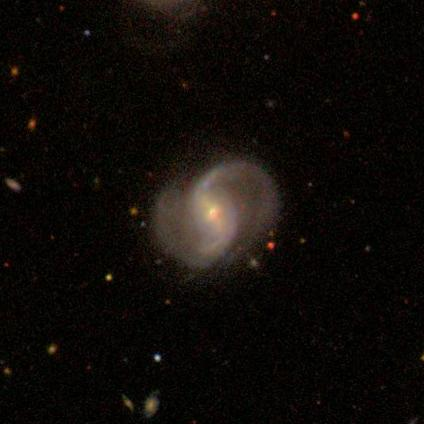
\includegraphics[width=0.9\textwidth]{Figures/137506.jpg}
            \caption{An image of a spiral galaxy direct from one of the catalogues of classified galaxies}
            \label{fig:137506}
        \end{figure}
        \end{column}
    \end{columns}
    \end{frame}


\subsection{Theory}
\begin{frame}{Morphology}
    \begin{alertblock}{}
    \begin{itemize}
        \item The Hubble scheme is primarily used for classifying
        \item Split into Elliptical galaxies, Spiral galaxies, and then a couple more smaller categories.
        \item Spiral galaxies arranged based on the presence of a bar, and then the tightness of their arms.
    \end{itemize}
    \end{alertblock}
    \begin{figure}
        \centering
        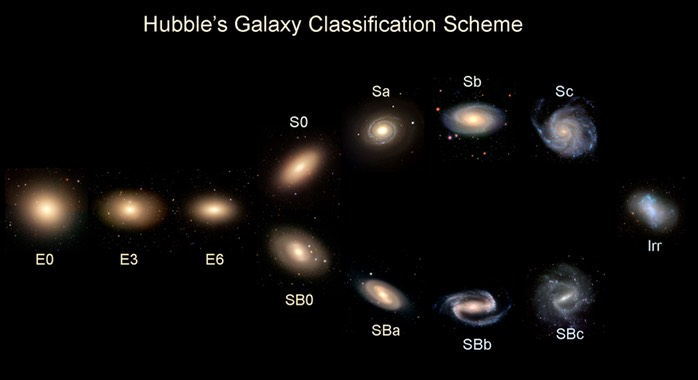
\includegraphics[width=0.8\textwidth, height=0.4\textheight]{Figures/hubbletuningfork.jpeg}
        \caption{Hubble 'Tuning Fork' Diagram, showing the different galaxies separated by their observable features}
        \label{fig:htuning}
    \end{figure}
    
\end{frame}

\begin{frame}{}
        \begin{columns}
        \begin{column}{0.45\textwidth}
        \begin{figure}
            \centering
            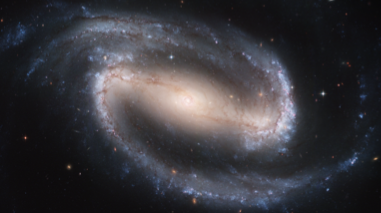
\includegraphics[width=\textwidth]{Figures/NGC1300.png}
            \caption{NGC1300, a barred galaxy}
            \label{fig:1300}
        \end{figure}
        \end{column}
        \begin{column}{0.45\textwidth}
        \begin{figure}
            \centering
            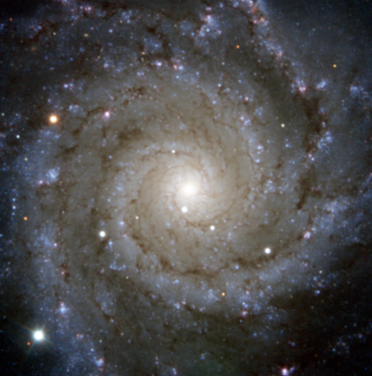
\includegraphics[width=\textwidth]{Figures/NGC638.png}
            \caption{NGC628, an unbarred galaxy}
            \label{fig:628}
        \end{figure}
        
        \end{column}
        \end{columns}
\end{frame}


\begin{frame}{Machine Learning Methods}
    \begin{block}{}
    \begin{itemize}
        \item Machine learning is incredibly diverse as a field.
        \item Within this project I used the methods for image recognition, Neural Networks.
        \item Networks 'look' at an image, identify features and classify based on these.
    \end{itemize}
    \end{block}
    \begin{columns}
    \begin{column}{0.5\textwidth}
    \begin{figure}
        \centering
        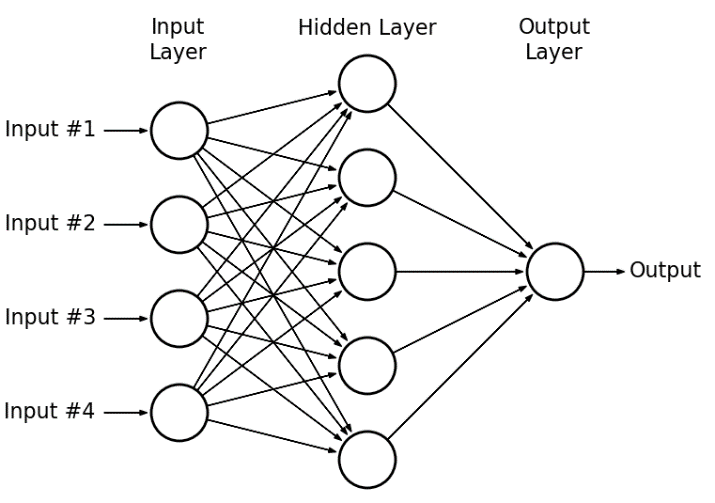
\includegraphics[width=\textwidth, height=0.4\textheight]{Figures/MLP.png}
        \caption{The simplest neural network, a Multi-layer Perceptron}
        \label{fig:MLP}
    \end{figure}
    \end{column}
    \begin{column}{0.5\textwidth}
    \begin{figure}
        \centering
        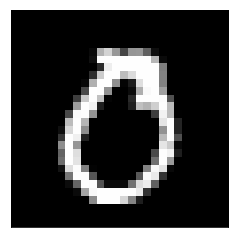
\includegraphics[width=0.8\textwidth, height=0.4\textheight]{Figures/MNIST_44_0.png}
        \caption{Some images from the MNIST dataset of handwritten digits}
        \label{fig:mnist}
    \end{figure}
    \end{column}
    \end{columns}
\end{frame}

\begin{frame}{Convolutional Neural Networks}
    \begin{figure}
        \centering
        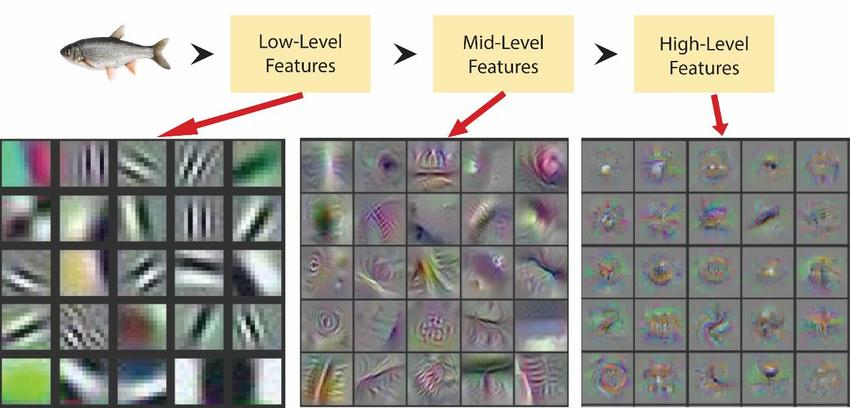
\includegraphics[width=\textwidth]{Figures/CNNfMap.png}
        \caption{Simple to complex feature extraction by a CNN where the initial layer detects simple patterns like edges and corners while higher layers detect more abstract features}
        \label{fig:cnnfmap}
    \end{figure}
    
\end{frame}

\begin{frame}{Convolutional Neural Networks}
    \begin{figure}
        \centering
        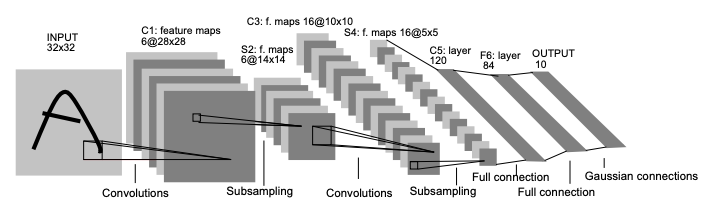
\includegraphics[width=\textwidth]{Figures/LeNet-5.png}
        \caption{The architecture for LeNet-5, a CNN for digit recognition}
        \label{fig:lenet5}
    \end{figure}
    
\end{frame}


\subsection{Method}
\begin{frame}{Starting Off}
    \begin{columns}
    \begin{column}{0.5\textwidth}
    \begin{figure}
        \centering
        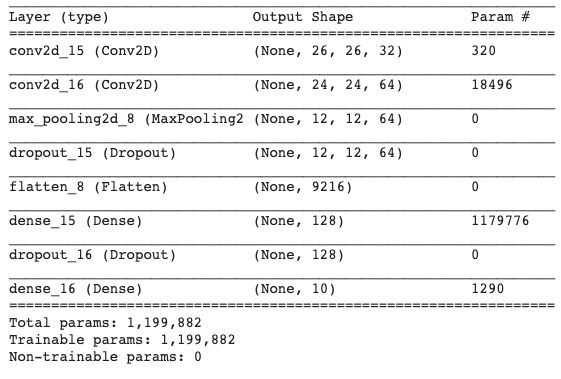
\includegraphics[width=\textwidth]{Figures/simplenetwork.png}
        \caption{A simple network I built towards the start of the project}
        \label{fig:simplenetwork}
    \end{figure}
    \end{column}
    \begin{column}{0.5\textwidth}
    \begin{figure}
        \centering
        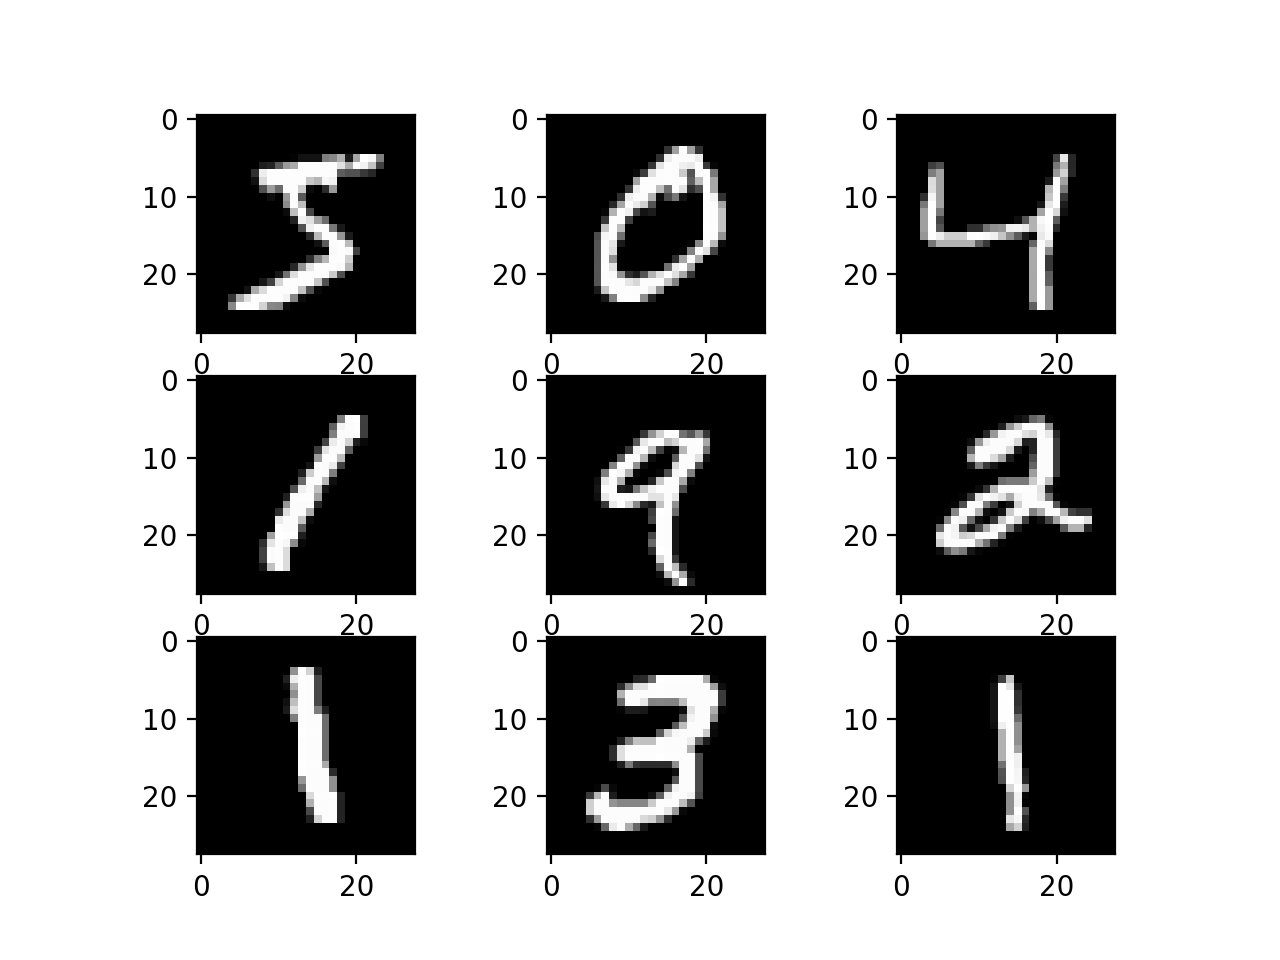
\includegraphics[width=\textwidth]{Figures/MNIST_Image.png}
        \caption{Some images from the MNIST dataset of handwritten digits}
        \label{fig:mnist}
    \end{figure}
    \end{column}
    \end{columns}
\end{frame}


\begin{frame}{The Data}

    \begin{figure}
        \centering
        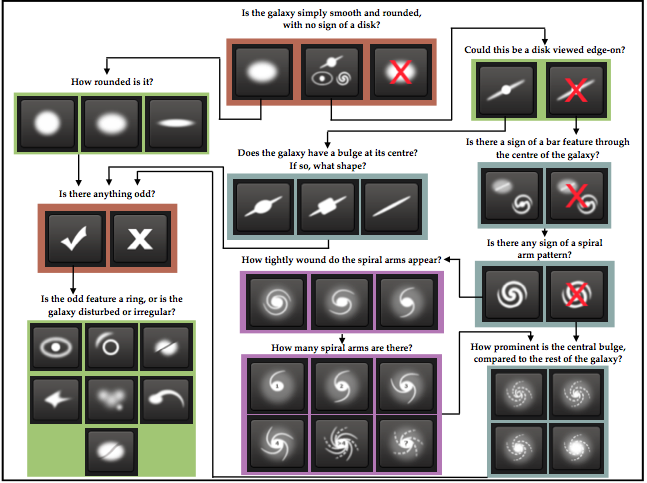
\includegraphics[width=0.7\textwidth]{Figures/GZ_Decison_Tree.png}
        \caption{The decision tree of questions posed to users of the Galaxy Zoo 2 project to classify galaxies }
        \label{fig:gztree}
    \end{figure}

\end{frame}




\begin{frame}{My Implementation}
    \begin{columns}
    \begin{column}{0.6\textwidth}
    \begin{block}{}
    \begin{itemize}
        \item The Galaxy Zoo data set is relatively small, and can lead to issues where the network doesn't generalise well to new data.
        \item I implemented a method called Transfer Learning.
        \item This looks at pre-training the network to improve generalisation.
    \end{itemize}
    \end{block}
    \end{column}
    \begin{column}{0.4\textwidth}
    \begin{figure}
        \centering
        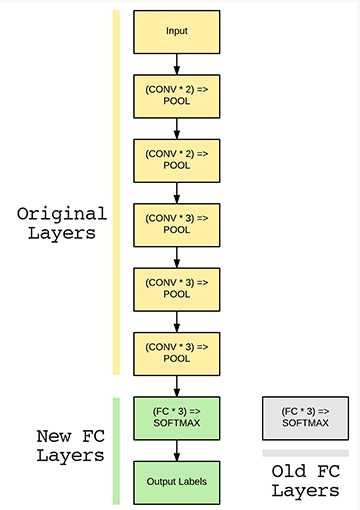
\includegraphics[width=.9\textwidth, height =0.6\textheight]{Figures/transferpic.png}
        \caption{An example of how transfer learning is applied}
        \label{fig:transferlearn}
    \end{figure}
    \end{column}
    \end{columns}
\end{frame}

\begin{frame}{The Project}
    \begin{alertblock}{}
    \begin{itemize}
        \item This research is still ongoing, but will once finished will serve as a proof of concept for the use of transfer learning.
        \item The project has challenged me in a variety of ways.
        \item I wrote a 25 page report as a pre-cursor to this project.
        \item I taught myself about the whole topic, as well as how to build NN's in Python.
        \item Developed my project management skills through the use of a logbook and project plan.
    \end{itemize}
    \end{alertblock}
\end{frame}



\subsection{}
\begin{frame}{}
    \begin{center}
        Thank you for listening, any questions?
    \end{center}
\end{frame}


\bibliographystyle{plain}
\bibliography{ref.bib}
\end{document}